% Proactive Feasibility Scheduling -- v3.5 manuscript
%
% REFRAMED (v3.4). Earlier versions presented this work as "we propose an ML
% scheduler that beats FIFO". The v3.3 baseline study and the v3.4 experiments
% below no longer support that framing, so the paper is now what the evidence
% actually is: an evaluation study and a negative result about using a learned
% wait-time regressor as a queue-ordering score.

\documentclass[11pt,twocolumn]{article}

\usepackage[utf8]{inputenc}
\usepackage[margin=0.9in]{geometry}
\usepackage{cite}
\usepackage{amsmath}
\usepackage{amssymb}
\usepackage{graphicx}
\usepackage{color}
\usepackage{xcolor}
\usepackage{listings}
\usepackage{hyperref}
\usepackage{booktabs}
\usepackage{fancyhdr}

\pagestyle{fancy}
\fancyhf{}
\fancyhead[C]{\small Ranking Degeneracy in ML-Based Job Scheduling}
\fancyfoot[C]{\thepage}

\title{Ranking Degeneracy: A Learned Wait-Time Model Schedules\\
       No Better Than Sorting by Requested Size}

\author{
  Rakshit Rameshbabu \\
  \small Vellore Institute of Technology, Chennai
}

\date{\today}

\begin{document}

\maketitle

\begin{abstract}
A common recipe in ``ML for systems'' is to train a regressor that predicts job
wait time from cluster-state features and then use its predictions to order the
queue. We report that this recipe is \emph{structurally degenerate}. At any
single dispatch instant every queued job observes the same cluster, so in the
feature vector only the job's own attributes differ, and in the standard
cluster-state feature set every such attribute is a deterministic function of
the job's requested size. The learned score is therefore a function of
requested size alone, and the ordering it induces is a per-instant lookup table
from size to priority: the cluster-state features shift all scores equally and
cannot reorder anything. We verify this over $45{,}432$ dispatch instants in three
settings --- $41{,}786$ replayed from two Parallel Workloads Archive traces and
$3{,}646$ from a synthetic generator --- and find zero counterexamples --- two jobs of equal size never receive
different scores. The consequences are measurable. On the synthetic benchmark a
one-line sort by requested size is statistically \emph{equivalent} to the full
XGBoost pipeline (paired TOST $p = 2.6\times10^{-16}$, difference CI
$[+0.03, +0.23]$ ts against a $\pm 1.59$ ts margin), and an MLP on the same
features reproduces the size sort exactly. We then re-ask the whole scheduler
comparison on two real traces, replacing the simulated user-estimate model with
the estimates the traces actually contain. The synthetic $7.9\%$ mean-wait gain
over FCFS does not replicate: the ML scheduler is indistinguishable from FCFS on
LANL CM-5 ($p = 0.48$) and any classical policy with a runtime estimate beats it
on both machines. \emph{As a second and independent contribution} --- independent
because it concerns the estimate-error model rather than the ranking score --- we
measure real user-estimate error against the $f$-model that the backfill
literature assumes, and find real error far more damaging to backfill than the
over-estimate-only $f$-model predicts ($+74\%$ mean wait on
LANL, where $36.3\%$ of user estimates are \emph{under}-estimates that the
$f$-model cannot generate at all). We argue the failure is one of feature design rather
than model class, state the condition a wait-time feature set must satisfy to be
non-degenerate, and release the harness, traces, and seeds.
\end{abstract}

\section{Introduction}

Machine learning for cluster scheduling is an active area, and a recurring
design is: (i) log cluster state, (ii) train a regressor to predict a job's wait
time, (iii) at each scheduling decision, score the queued jobs with the
regressor and dispatch in ascending predicted wait. The intuition is that a
model which has seen how the queue evolves can anticipate contention better than
a fixed heuristic.

This paper reports that step (iii) does not do what it appears to do. The
argument is elementary but, as far as we can tell, not stated in the literature
we build on, and it invalidates the natural reading of any improvement measured
this way.

\paragraph{The degeneracy.}
Fix a dispatch instant $t$ with cluster state $S_t$ and queue $Q_t$. The feature
vector for job $j$ splits into two groups: features of the machine (free
processors, queue length, number of running jobs, fragmentation, queue pressure)
and features of the job (requested size, and quantities derived from it such as
``does it fit now''). The first group is \emph{identical for every job in
$Q_t$} --- it describes $S_t$, not $j$. So for two jobs $j_1, j_2 \in Q_t$ the
predicted waits can differ only through the second group. In the 12-feature set
used here (and in the 8-feature set reconstructible from a Standard Workload
Format trace) every member of the second group is a deterministic function of the
requested size $g_j$ once $S_t$ is fixed:
\begin{align*}
\texttt{can\_fit\_now} &= \mathbb{1}[\,\text{free}(S_t) \ge g_j\,] \\
\texttt{gpu\_fit\_ratio} &= \min(\text{free}(S_t)/g_j,\; 1) \\
\texttt{node\_availability} &= |\{n : \text{free}_n(S_t) \ge g_j\}| / N \\
\texttt{queue\_pressure} &= (\Sigma_{Q_t} - g_j)/(\text{free}(S_t)+1).
\end{align*}
Hence the score satisfies
\[
  \widehat{w}(j \mid S_t) \;=\; g_{S_t}(g_j)
\]
for some function $g_{S_t}$ determined entirely by the state, and the induced
queue order is the order of $g_{S_t}$ over the sizes present in $Q_t$. The model
is, at each instant, a \emph{lookup table from requested size to priority}. The
remaining seven features describe only the cluster --- they select \emph{which}
table is used --- but they cannot distinguish two co-queued jobs, which is the
only thing a ranking consumes. (\texttt{queue\_pressure} does differ between
co-queued jobs, but only through the $-g_j$ term: it is itself a function of
size given the state, so it cannot break the degeneracy.)

\paragraph{Why this matters.}
If the argument holds, then a reported improvement of an ML wait-time scheduler
over FCFS is evidence about size-based ordering, not about learning. The correct
control is not FIFO; it is \emph{sorting by requested size}, which needs no
dataset, no training, no inference, no SHAP explanation, and no drift monitor.
To our knowledge that control is absent from the ML-scheduling evaluations we
are aware of, including our own earlier versions of this work.

\paragraph{A second contribution.}
The trace-driven re-evaluation required us to replace the simulated
user-estimate model with the estimates the traces actually contain, and that
substitution turned out to carry a finding of its own, independent of the
degeneracy. The standard $f$-model, $\hat r = r\cdot f$ with $f \sim U(1,C)$,
can only over-estimate. Real estimates on LANL CM-5 are under-estimates
$36.3\%$ of the time, and under-estimates break the very mechanism EASY
backfilling relies on: EASY with real estimates costs $+74\%$ mean wait against
perfect estimates on LANL, where the $f$-model predicts near-insensitivity.
This is a statement about how backfill should be evaluated, not about ML, and we
report it as a second contribution (\S\ref{sec:estimates}) rather than as a
by-product of the first.

\paragraph{Contributions.}
\begin{enumerate}
  \item \textbf{The degeneracy, stated and measured} (\S\ref{sec:degeneracy}).
        Over $45{,}432$ dispatch instants across a synthetic generator and two
        real traces, two equally-sized co-queued jobs never receive different
        scores (0 violations). Seven of the twelve features vary across the
        queue in $0.0\%$ of instants, and every feature that does vary is a
        deterministic function of the requested size. A nine-job queue receives
        only $2.3$--$3.1$ distinct priority levels.
  \item \textbf{An equivalence result, not a null result}
        (\S\ref{sec:equivalence}). Using paired TOST rather than a failure to
        reject, sorting by requested size is statistically equivalent to the
        XGBoost scheduler on the synthetic benchmark
        ($p_{\mathrm{TOST}} = 2.6\times10^{-16}$) and on SDSC SP2
        ($p_{\mathrm{TOST}} = 1.8\times10^{-12}$). An MLP over the same features
        reproduces the size sort \emph{exactly} on all 20 paired runs.
  \item \textbf{A trace-driven re-evaluation} (\S\ref{sec:traces}). Replaying
        LANL CM-5 and SDSC SP2 through twelve policies, with the real user
        runtime estimates the traces contain, the synthetic $7.9\%$ gain over
        FCFS does not replicate, and every policy with access to a runtime
        estimate beats the ML scheduler on both machines.
  \item \textbf{Second contribution: real estimate error breaks backfill far
        more than the $f$-model suggests} (\S\ref{sec:estimates}). Real estimates are
        $6.9\times$ the runtime at the median on SDSC but only $1.5\times$ on
        LANL, where $36\%$ are \emph{under}-estimates --- a case the standard
        over-estimate-only $f$-model cannot produce. Backfill costs $+74\%$ mean
        wait on LANL under real estimates versus perfect ones, against near-zero
        sensitivity under the $f$-model.
  \item \textbf{A non-degeneracy condition and a reproducible harness}
        (\S\ref{sec:fix}). We state what a feature set must contain to make
        learning matter for ranking, and release code, traces, and seeds.
\end{enumerate}

\section{Related Work}

\paragraph{Predicting queue wait time.}
Wait-time prediction for batch queues is long-standing: Downey's log-uniform
lifetime models, template-based prediction from historical similar jobs, and the
QBETS/Karnak line of quantile-based bound predictors all predate modern ML
pipelines \cite{Feitelson1997, Feitelson2011}. The recent line is explicitly
ML-based. Park \cite{Park2019} predicts queue wait on a national
supercomputer; Lovell et al.\ \cite{Lovell2024} use a hierarchical deep model
for the same task; Ramachandran et al.\ \cite{Ramachandran2024} combine
regressors with metaheuristic hyper-parameter search; and Barsanti and Sodan
\cite{Barsanti2006} use predicted wait to drive adaptive resource allocation.
Our contribution is not a better predictor. It is an observation about what
happens when any such predictor is used as a \emph{ranking} score, and it
applies to this whole line: the relevant question for each is whether the
feature set contains a per-job attribute that is not a function of requested
size given the cluster state (\S\ref{sec:fix}).

\paragraph{Why reported gains over FIFO and this result are compatible.}
Many ML-for-systems papers report real gains against a first-in-first-out
baseline, and nothing here contradicts them. Our claim is narrow in three ways,
and a reported gain can sit outside all three. First, it concerns
\emph{ranking}: a learned component that drives \emph{admission}, \emph{placement},
or \emph{backfill} selection is choosing among actions the queue order does not
determine, and the degeneracy argument --- which is about separating two
co-queued jobs --- says nothing about it. The deep-RL policies of Mao et al.\
\cite{ML-Scheduling1, ML-Scheduling2} are of this kind, as is the learned-index
line in databases \cite{Kraska2018}, where the learned object replaces a
structure rather than a comparator. Second, it concerns a \emph{feature family}:
a feature set containing a genuine per-job attribute --- a runtime estimate, an
application signature, a model-level descriptor as in Wang et al.\
\cite{Wang2023} --- is non-degenerate by Proposition~2, and a gain measured with
such a feature set is a gain from that attribute. Third, it concerns the
\emph{control}: our result says the correct comparison for a degenerate feature
set is sorting by size, not FIFO, and a gain over FIFO is simply silent about
whether the size sort would have delivered it. So the claim compatible with both
literatures is not ``ML does not help scheduling'' but ``a gain over FIFO does
not localise the mechanism''. Marcus et al.\ \cite{Marcus2020} make the
corresponding point for learned indexes by benchmarking them against carefully
tuned classical structures rather than against naive ones.

\paragraph{Learning to rank.}
Because the output we criticise is an ordering, the learning-to-rank literature
\cite{Burges2005, Liu2009} is the natural place to look for an escape: replace
the pointwise regression objective with a pairwise or listwise one that
optimises the ordering directly. It does not escape. Proposition~1 constrains
the feature map, not the loss, and we verified this empirically: an XGBoost
ranker trained with \texttt{rank:pairwise} and one trained with
\texttt{rank:ndcg} over the same features both produce \emph{zero}
counterexamples on both traces, as do monotone reshapings of the pointwise score
(\S\ref{sec:scope}). A pairwise objective learns which of two jobs should go
first; when the two jobs present identical feature vectors, there is nothing for
it to learn from. This is worth stating because ``we used a ranking loss'' is the
most plausible objection to the result, and it is measurably not a fix.

\paragraph{Backfilling and user runtime estimates.}
Backfilling \cite{SLURM2003} is the dominant production technique. EASY
\cite{Mualem2001} reserves capacity for the queue head and backfills jobs that
either finish before the reservation or fit in the surplus beyond the head's
requirement. Conservative backfill reserves for every queued job. Variants
refine which job to pick and how much slack to allow: lookahead
\cite{Shmueli2003}, slack-based priority \cite{Talby1999}, adaptive reservation
\cite{Shmueli2005}, probabilistic backfilling on predicted-runtime
distributions \cite{Nissimov2007}, and deviation backfilling \cite{Hai2023}.
All depend on user runtime estimates, and our \S\ref{sec:estimates} is in direct
dialogue with two papers in particular. Mu'alem and Feitelson \cite{Mualem2001}
define the two-condition EASY rule we implement and introduce the $f$-model,
$\hat r = r\cdot f$ with $f\sim U(1,C)$, as the standard way to inject estimate
error into a backfill evaluation. Our point is that this model is not merely
imprecise but \emph{structurally} unable to express the failure mode we measure:
$f \ge 1$ means $\hat r \ge r$ always, so an $f$-model evaluation contains no
under-estimates by construction, while $36.3\%$ of LANL's real estimates are
under-estimates. An under-estimate is precisely what invalidates EASY's
reservation --- a job admitted on the promise that it will finish before the
reservation, and does not, delays the queue head --- so the one error direction
the model omits is the one that breaks the mechanism. Tsafrir et al.\
\cite{Tsafrir2005} model user estimates in detail and, with Mu'alem and
Feitelson, report the counter-intuitive finding that over-estimation can
\emph{help} backfill by making the scheduler conservative; we do not dispute
that, and it is consistent with SDSC, where estimates are $6.9\times$ runtime at
the median and EASY loses only $6.2\%$ against perfect estimates. Our claim is
that this benign regime is not universal: LANL, roughly calibrated at the median
($1.5\times$) but with a third of estimates too low, costs EASY $+74\%$. The
literature's own methodological warning applies to itself here --- Feitelson
\cite{Feitelson2005} shows how strongly backfilling conclusions depend on
exactly such evaluation choices --- and we read our result as an instance of
that warning rather than as a contradiction of \cite{Mualem2001, Tsafrir2005}.
Tsafrir et al.'s later move to system-generated predictions \cite{Tsafrir2007}
is the constructive response, and it sidesteps the $f$-model question entirely
by not using user estimates.

\paragraph{Replacing user estimates with predictions.}
The closest prior work replaces the user's estimate with a system-generated one.
Tsafrir et al.\ \cite{Tsafrir2007} predict runtimes from user history and
backfill on the prediction; Minh and Wolters \cite{Minh2010} predict application
runtimes from historical data for the same purpose; Park and Hong
\cite{Park2025} improve runtime prediction by conditioning on application type.
Yuan et al.\ \cite{Yuan2014} note that naively feeding predictions into EASY
causes reservation violations and add fairness guarantees to prevent it. This
line differs from ours in the quantity predicted: a runtime estimate is a
genuine per-job attribute, so ordering by it is \emph{not} degenerate --- which
is precisely why \textsc{Sjf\_UserEst} beats the wait-time model in
\S\ref{sec:traces}, and why a runtime estimate is our first suggested fix.

\paragraph{Learning-based schedulers.}
Deep-RL approaches \cite{ML-Scheduling1, ML-Scheduling2} learn a policy
end-to-end rather than fitting a regressor and sorting by it, and so are not
subject to the degeneracy as stated --- though the same question (what is the
ML-free control?) applies to them. Wang et al.\ \cite{Wang2023} schedule ML
cluster jobs from model-level features, an example of a feature set that
\emph{does} carry per-job information beyond size. Hovestadt et al.\
\cite{Hovestadt2003} frame the underlying choice as queueing versus planning.

\paragraph{Workloads and metrics.}
Our synthetic substrate is a simple generator, not a validated workload model;
Lublin and Feitelson \cite{Lublin2003}, Downey and Feitelson \cite{Downey1999},
and Feitelson and Shmueli \cite{Feitelson2009} give the principled alternatives,
and \S\ref{sec:threats} treats this as a limitation. Zhang et al.\
\cite{Zhang2024} report cross-system variation in job characteristics of the
kind that produces our LANL-versus-SDSC divergence. Bounded slowdown
\cite{Feitelson2000} and Jain's index \cite{Jain1984} are the standard
evaluation metrics; we report both, having found that mean wait alone hides the
effect on short jobs. Goponenko et al.\ \cite{Goponenko2022} argue that these
metrics correlate poorly with packing and fairness objectives, which is
consistent with the metric-dependent verdicts we obtain in
\S\ref{sec:equivalence}.

\paragraph{Negative results, weak baselines, and reproducibility.}
The justification for publishing this at all comes from a literature about how
empirical progress is measured. Armstrong et al.\ \cite{Armstrong2009} showed
that a decade of reported retrieval improvements largely failed to accumulate
because each was measured against a weak baseline; Lin \cite{Lin2018} and
Dacrema et al.\ \cite{Dacrema2019} found the same pattern in neural retrieval
and neural recommendation, the latter reproducing eighteen published methods and
finding most beaten by well-tuned non-neural baselines; Musgrave et al.\
\cite{Musgrave2020} report the analogous result for deep metric learning; and
Sculley et al.\ \cite{Sculley2018} argue that empirical rigour, not pace, is the
binding constraint. Our finding is the batch-scheduling instance of exactly this
failure mode, with an unusually clean diagnosis: the appropriate strong baseline
is not merely well-tuned, it is \emph{derivable from the model's own feature
set}, and it is a one-line sort. We also follow this literature in method ---
equivalence testing rather than a failed difference test
(\S\ref{sec:equivalence}), and reporting the split the accuracy number actually
came from (\S\ref{sec:threats}) --- and in artefact practice, since Collberg and
Proebsting \cite{Collberg2016} document how rarely systems results can be
re-run at all. Every number in this paper is produced by a single seeded
pipeline whose per-step provenance is cited in each table and figure caption.
A negative result is only worth reading if it can be checked.

\section{Experimental Setup}

\subsection{Two evaluation substrates}

\paragraph{Synthetic (for continuity).}
A discrete-time simulator: 8 nodes $\times$ 4 GPUs, 110 jobs arriving uniformly
over the first 150 of 300 timesteps, sizes $U\{1,8\}$, runtimes $U\{5,20\}$. 20
paired runs (seeds $1000{+}i$, disjoint from the model's training seeds
$42{+}i$). This is the substrate all earlier versions of this work used, and we
keep it only so the new controls can be compared against the previously
published numbers.

\paragraph{Trace-driven (for validity).}
Two cleaned Parallel Workloads Archive traces: LANL CM-5 (1994, 1024
processors, $122{,}055$ kept jobs) and SDSC SP2 (1998, 128 processors,
$43{,}117$ kept jobs). We reserve the first $60\%$ of each trace's time span for
model training and carve 20 evenly spaced evaluation windows from the remainder,
each 3 simulated days of warm-up (not measured) followed by 7 measured days.
Mean offered load is $0.72$ (SDSC) and $0.68$ (LANL). Windows are evenly spaced,
\emph{not} selected by load, to avoid cherry-picking congestion.

The trace simulator is event-driven and exact to the second: state changes only
at arrivals and completions, so there is no tick-quantisation bias. Because SWF
records no per-node placement, we model capacity only; inventing node-level
fragmentation would be fabricating data. \S\ref{sec:threats} reports the
resulting fidelity gap.

\subsection{Policies}

Twelve policies. \textsc{FCFS} (first-come first-served with unrestricted
first-fit), \textsc{Fifo\_Strict} (a blocked head blocks the queue),
\textsc{Sjf\_Oracle} (true runtimes; unattainable), \textsc{Sjf\_UserEst} (the
trace's real requested time), \textsc{Hrrn\_UserEst}, \textsc{Smallest\_First}
(sort by requested size --- the degeneracy control), \textsc{Easy\_UserEst} and
\textsc{Easy\_Oracle} (canonical two-condition EASY),
\textsc{Cons\_Bf\_UserEst}, \textsc{Srpt\_Oracle} (preemptive, with a
checkpoint penalty charged as waiting), \textsc{Proactive} (the XGBoost
wait-time model, retrained per trace, no runtime information), and
\textsc{Proactive\_Est} (the same model retrained with the user estimate as an
extra feature --- the control for ``does ML add anything beyond the estimate?'').

The ML scheduler is given its best case throughout: a model retrained on the
same machine's own earlier data. Zero-shot transfer from the synthetic generator
to these traces yields $R^2 \approx 0$ and is not a competitive configuration.

\subsection{Metrics and statistics}

We report mean wait, p95 wait, \textbf{mean bounded slowdown}
$\max(\text{turnaround}/\max(r, \tau), 1)$ with $\tau = 60$s
\cite{Feitelson2000}, the Gini coefficient of waits, and utilisation. Wait is
defined uniformly as turnaround minus true runtime, so preemptive requeue time
and checkpoint overhead are charged to the preemptive policy rather than hidden.

Comparisons are paired (same workload, every policy) with Holm-adjusted
$t$-tests and Wilcoxon signed-rank tests. Crucially, claims that two policies
perform \emph{the same} use paired TOST equivalence tests with a margin of
$10\%$ of the reference mean; a large $p$-value from a difference test is not
evidence of equivalence, and treating it as such is how a degenerate policy
survives review.

\section{The Ranking Degeneracy, Measured}
\label{sec:degeneracy}

We instrumented every \textsc{Proactive} ranking decision in real simulations
($45{,}432$ instants with $\ge 2$ queued jobs) and recorded, per instant, which
features differ across the queue and how the resulting order compares with
ML-free orders. Table~\ref{tab:degeneracy} summarises, and
Figure~\ref{fig:degeneracy} shows the per-feature variation directly.

\begin{table}[h]
\centering
\footnotesize
\begin{tabular}{lrrr}
\toprule
 & Synthetic & SDSC & LANL \\
\midrule
Ranking instants        & 3{,}646 & 11{,}843 & 29{,}943 \\
Features (total)        & 12 & 8 & 8 \\
Features varying (mean) & 2.62 & 2.87 & 2.69 \\
Equal size, diff.\ score & \textbf{0} & \textbf{0} & \textbf{0} \\
Distinct scores / queue & 2.81 & 3.09 & 2.28 \\
Kendall $\tau$ vs.\ size & 0.71 & 0.75 & 0.62 \\
Order $=$ smallest-first & 80.3\% & 71.5\% & 77.6\% \\
Order $=$ arrival (FCFS) & 19.7\% & 18.1\% & 27.5\% \\
Size table monotone     & 63.1\% & 57.1\% & 56.9\% \\
\bottomrule
\end{tabular}
\caption{The learned score never distinguishes two equally-sized co-queued jobs.
Cluster-state features vary across the queue in $0.0\%$ of instants.
{\small Source: \texttt{05\_results/degeneracy/ranking\_degeneracy.csv} and
\texttt{05\_results/degeneracy/feature\_variation.csv}, produced by
\texttt{python 04\_scheduler/ranking\_degeneracy.py} (step 9 of
\texttt{run\_all\_experiments.sh}).}}
\label{tab:degeneracy}
\end{table}

\begin{figure*}[t]
\centering
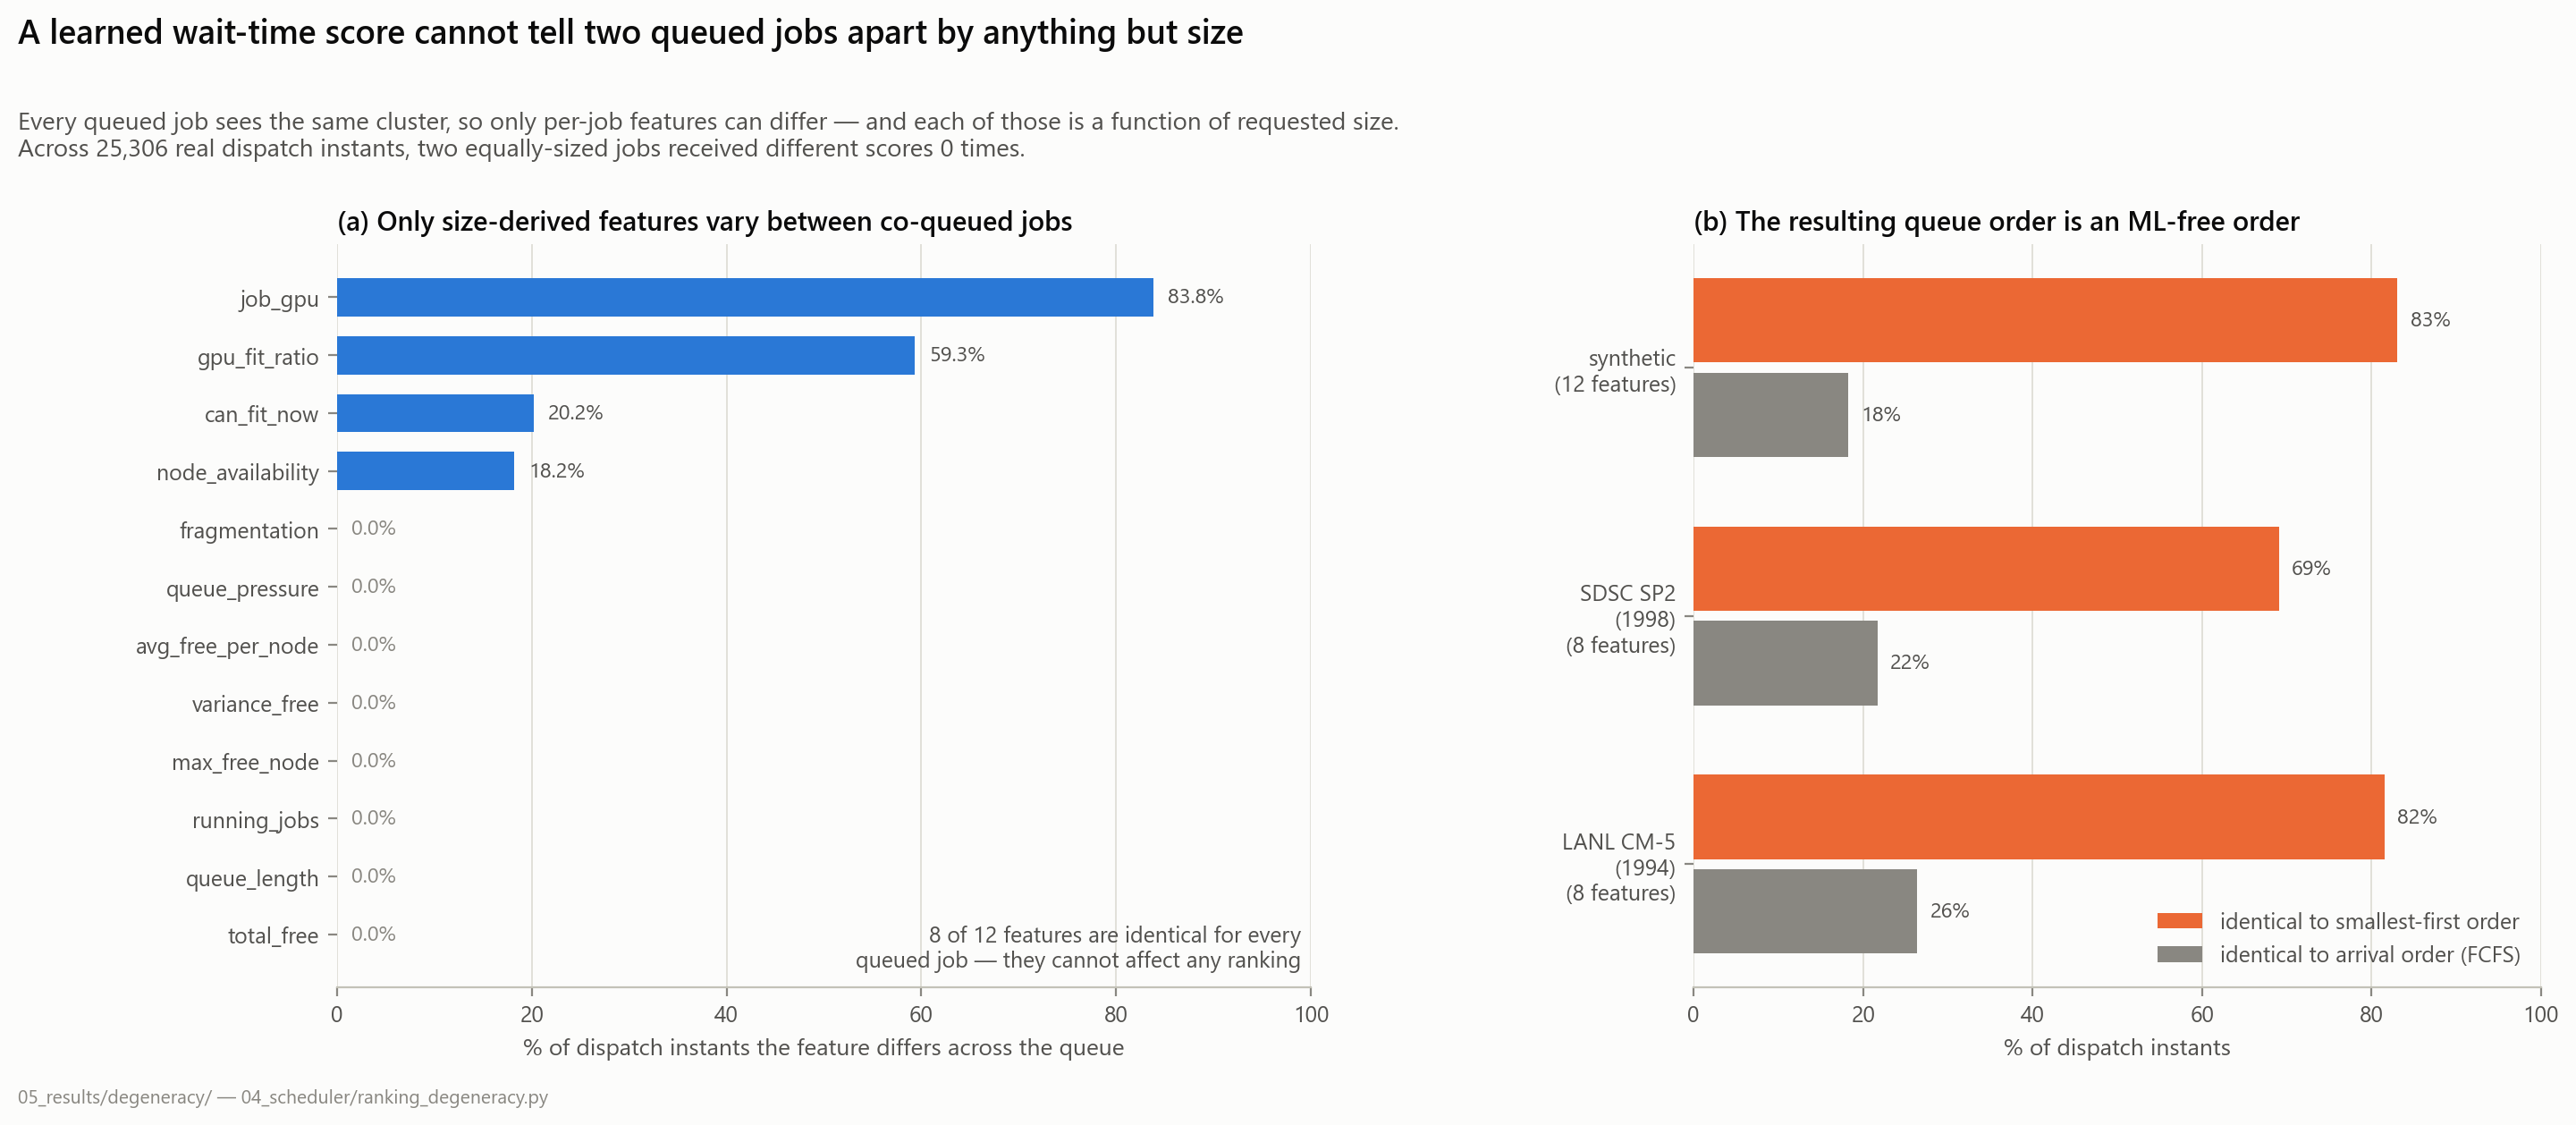
\includegraphics[width=\textwidth]{../../05_results/degeneracy/ranking_degeneracy.png}
\caption{Feature variation in ranking decisions. What to look for: the bars for
the seven cluster-state features sit flat on zero --- they do not vary across a
queue in \emph{any} instant --- while the only bars with any height belong to
the job's requested size and to the four quantities derived from it. The reader
should also see that the same shape recurs in all three settings, so the
degeneracy is not an artefact of one substrate.
{\small Source: \texttt{05\_results/degeneracy/ranking\_degeneracy.png},
plotted from \texttt{05\_results/degeneracy/feature\_variation.csv} and
\texttt{05\_results/degeneracy/ranking\_degeneracy.csv}, produced by
\texttt{python 04\_scheduler/ranking\_degeneracy.py} (step 9 of
\texttt{run\_all\_experiments.sh}).}}
\label{fig:degeneracy}
\end{figure*}

Three observations. First, the \emph{zero} in row four is the claim: across
$45{,}432$ instants there is no counterexample, exactly as the argument in
\S1 requires. Second, of the twelve synthetic features only five ever differ
between co-queued jobs (\texttt{job\_gpu}, \texttt{gpu\_fit\_ratio},
\texttt{can\_fit\_now}, \texttt{node\_availability}, \texttt{queue\_pressure})
and all five are functions of the requested size; the remaining seven vary in
$0.0\%$ of instants and are therefore incapable of affecting any ranking. Third,
the resolution is very coarse: a queue of $\sim$9 jobs is partitioned into only
$2.3$--$3.1$ priority classes, and in $18$--$27\%$ of instants \emph{every}
queued job receives the same score, so the policy silently reduces to FCFS.

The recovered size$\rightarrow$priority table is monotone increasing in only
$57$--$63\%$ of instants. Where it is monotone the policy \emph{is}
smallest-job-first; where it is not, the model has learned a non-trivial size
preference. We note explicitly that this fraction does \emph{not} predict where
the equivalence of \S\ref{sec:equivalence} fires --- SDSC ($57.1\%$), where the
size sort is certified equivalent, and LANL ($56.9\%$), where it is not, are
statistically indistinguishable on it. Degeneracy is the claim this section
supports; the shape of the learned table is a description of it, not an
explanation of the downstream scheduling difference.
Figure~\ref{fig:size-table} shows the recovered tables themselves.

\begin{figure}[t]
\centering
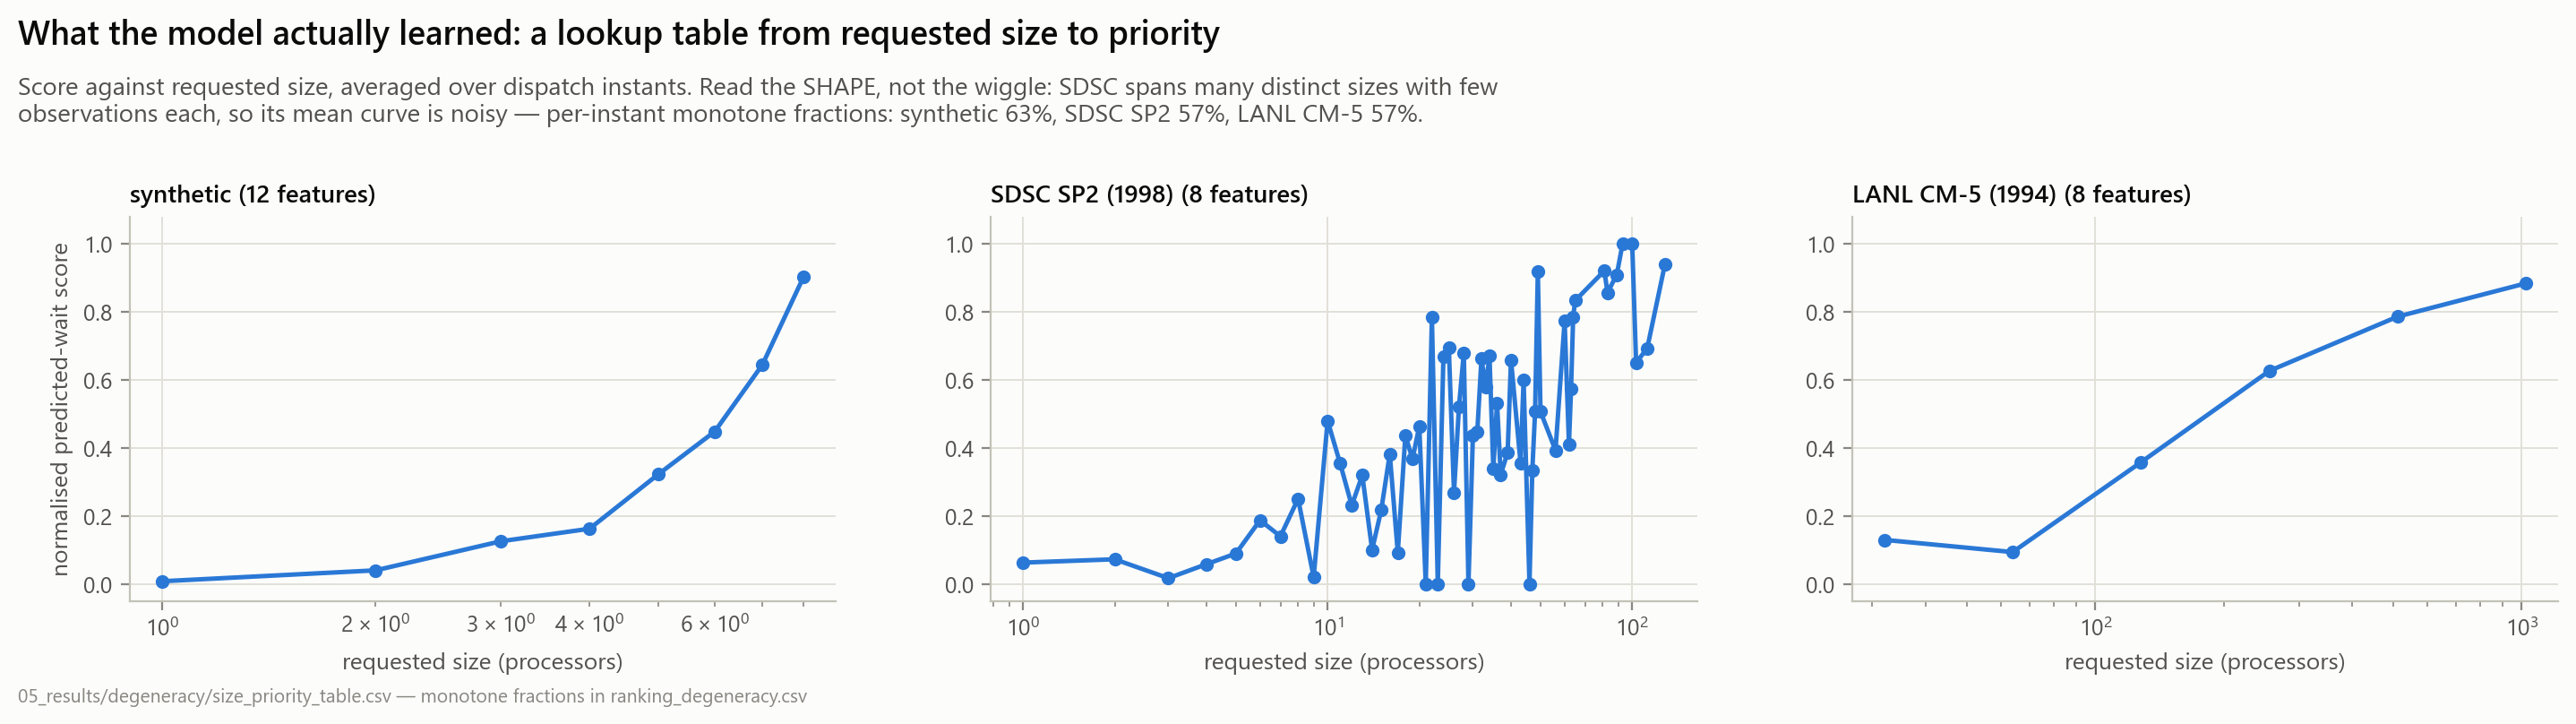
\includegraphics[width=\columnwidth]{../../05_results/degeneracy/size_priority_table.png}
\caption{The recovered size$\rightarrow$priority lookup table, per setting.
What to look for: each curve is a \emph{function} --- one priority per requested
size, which is the degeneracy --- but it is not always an \emph{increasing}
function. The synthetic curve climbs monotonically from $0.008$ at size 1 to
$0.902$ at size 8; the trace curves do not, dipping and rising instead (on SDSC,
size 3 scores $0.017$ against $0.072$ at size 2). That is exactly the
distinction Proposition~1 draws and its ``what it does not say'' note insists on:
degeneracy forces a table, it does not force smallest-first. Across instants the
table is monotone in only $63.1\%$ (synthetic), $57.1\%$ (SDSC) and $56.9\%$
(LANL) of cases.
{\small Source: \texttt{05\_results/degeneracy/size\_priority\_table.png},
plotted from \texttt{05\_results/degeneracy/size\_priority\_table.csv},
produced by \texttt{python 04\_scheduler/ranking\_degeneracy.py} (step 9 of
\texttt{run\_all\_experiments.sh}).}}
\label{fig:size-table}
\end{figure}

\subsection{The degeneracy, stated formally}
\label{sec:proposition}

Fix a dispatch instant $t$. Let $S$ denote the cluster state at $t$ --- free GPUs
per node, the running set, the queue contents, and any quantity derived from them
--- and let the queue be $Q=\{j_1,\dots,j_n\}$ with $g(j)$ the requested size of
job $j$. A feature map assigns to each queued job
$\varphi(j,S)=\bigl(\psi(j,S),\,\chi(S)\bigr)$, where $\chi(S)$ collects the
features that depend on the cluster alone and $\psi$ those that depend on the job.
A score function $f$ gives $s(j)=f(\varphi(j,S))$, and the dispatcher ranks $Q$ by
$s$ under a fixed tie-break.

\medskip
\noindent\textbf{Proposition 1 (ranking degeneracy).}
\emph{Suppose every per-job feature factors through the requested size given the
state: there is a map $\tilde\psi$ with $\psi(j,S)=\tilde\psi(g(j),S)$ for all
$j\in Q$. Then there exists $h_S$ with $s(j)=h_S(g(j))$ for all $j\in Q$.}

\medskip
\noindent\emph{Proof.} $\chi(S)$ does not depend on $j$, so at the fixed instant
$t$ it is a constant. Define $h_S(u):=f(\tilde\psi(u,S),\chi(S))$. Then for any
$j\in Q$, $s(j)=f(\tilde\psi(g(j),S),\chi(S))=h_S(g(j))$. \hfill$\square$

\medskip
\noindent\textbf{Corollary 1.1.} Every feature in $\chi$ enters $h_S$ as a constant
argument at a fixed instant, so it cannot separate two queued jobs, \emph{whatever}
$f$ is. No additivity or monotonicity assumption on $f$ is needed: the feature is
simply held fixed across the comparison. Seven of the twelve synthetic features are
of this kind, and they are measured to vary across a queue in $0.0\%$ of instants.

\medskip
\noindent\textbf{Corollary 1.2.} If $g(i)=g(j)$ then $s(i)=s(j)$. This is the
falsifiable form of the proposition, and it is what we count: zero counterexamples
over $45{,}432$ dispatch instants.

\medskip
\noindent\textbf{Corollary 1.3.} The number of distinct scores at an instant is at
most $|\{g(j):j\in Q\}|$. The induced order is therefore measurable with respect to
the partition of $Q$ into size classes: the policy may order size classes and can do
nothing within one. A queue of $8.5$--$10.2$ jobs receives $2.28$--$3.09$ distinct
priority levels, and every queued job receives an identical score in
$14.4$--$20.7\%$ of instants, where the policy is exactly FCFS.

\paragraph{What the proposition does not say.}
It does \emph{not} say the ranking is the ascending-size order. $h_S$ may order the
size classes arbitrarily; it may only not distinguish jobs within one. Our own
measurements make the distinction concrete: the recovered size-to-priority table is
monotone in just $57$--$63\%$ of instants, and Figure~\ref{fig:size-table} shows
tables that are plainly functions of size without being increasing in it. This is why we establish equivalence to a
size sort \emph{statistically}, by TOST against \textsc{Smallest-First}, rather than
deducing it. Degeneracy is a structural fact; that the resulting policy performs like
ascending-size order is a separate empirical claim.

\paragraph{The converse, and its limits.}
\textbf{Proposition 2.} \emph{If some per-job feature does not factor through
$(g,S)$ --- if $\psi(i,S)\neq\psi(j,S)$ is possible for two jobs with $g(i)=g(j)$ ---
then no such $h_S$ need exist and Corollary 1.2 can fail.} A feature set can produce
a ranking finer than the size partition only if it contains such an attribute. Three
limits bound what that buys. First, it is necessary but not sufficient:
\textsc{Proactive-Est} carries the user's runtime estimate, is non-degenerate by
Proposition 2, and still loses to plain SJF on both traces
(\S\ref{sec:traces}). Second, the attribute must be informative about wait, not
merely distinct --- a per-job nonce would break Corollary 1.2 while carrying no
information. Third, the shared-state premise is a modelling choice rather than a law:
a policy that scores a job when it \emph{enters} the queue and caches the result
violates it by construction, and whether such a policy schedules better is an
empirical question in which staleness is a cost as well as a source of variation.

\section{Sorting by Size Is Equivalent to the Model}
\label{sec:equivalence}

Table~\ref{tab:equiv} gives the paired TOST results.

\begin{table}[h]
\centering
\footnotesize
\setlength{\tabcolsep}{4pt}
\begin{tabular}{llrrl}
\toprule
Substrate & Metric & $\Delta$ & $p_{\mathrm{TOST}}$ & Eq.? \\
\midrule
Synthetic & mean wait & $+0.80\%$ & $2.6\times10^{-16}$ & equiv. \\
Synthetic & bnd.\ slow. & $+0.69\%$ & $3.8\times10^{-18}$ & equiv. \\
SDSC SP2  & mean wait & $-0.05\%$ & $1.8\times10^{-12}$ & equiv. \\
SDSC SP2  & bnd.\ slow. & $+2.7\%$ & $7.4\times10^{-4}$ & equiv. \\
LANL CM-5 & mean wait & $+14.4\%$ & $0.77$ & no \\
LANL CM-5 & bnd.\ slow. & $+7.3\%$ & $0.30$ & no \\
\bottomrule
\end{tabular}
\caption{\textsc{Smallest\_First} versus \textsc{Proactive}. $\Delta$ is the
difference in the metric (positive $=$ the size sort is worse). Equivalence
margin $10\%$ of the reference. ``Eq.?'' is the TOST verdict at that margin.
{\small Sources: \texttt{05\_results/schedulers/multi\_scheduler\_equivalence.csv},
produced by \texttt{python 04\_scheduler/multi\_scheduler\_benchmark.py}
(step 7 of \texttt{run\_all\_experiments.sh}), and
\texttt{05\_results/trace\_schedulers/trace\_scheduler\_equivalence.csv},
produced by \texttt{python 04\_scheduler/trace\_driven\_benchmark.py}
(step 10).}}
\label{tab:equiv}
\end{table}

On the synthetic benchmark the difference in mean wait is $+0.127$ ts with a
$90\%$ CI of $[+0.025, +0.228]$ against a $\pm 1.59$ ts margin: the entire
interval sits well inside the margin, so this is a positive finding of
equivalence, not an underpowered null. The MLP baseline is a sharper version of
the same point --- \textsc{NN} and \textsc{Smallest\_First} produce
\emph{bit-identical} results on every metric of all 20 runs. Two different model
classes over the same features collapse to the same one-line sort.
Figure~\ref{fig:synth-schedulers} places both against the wider synthetic
scheduler landscape.

\begin{figure}[t]
\centering
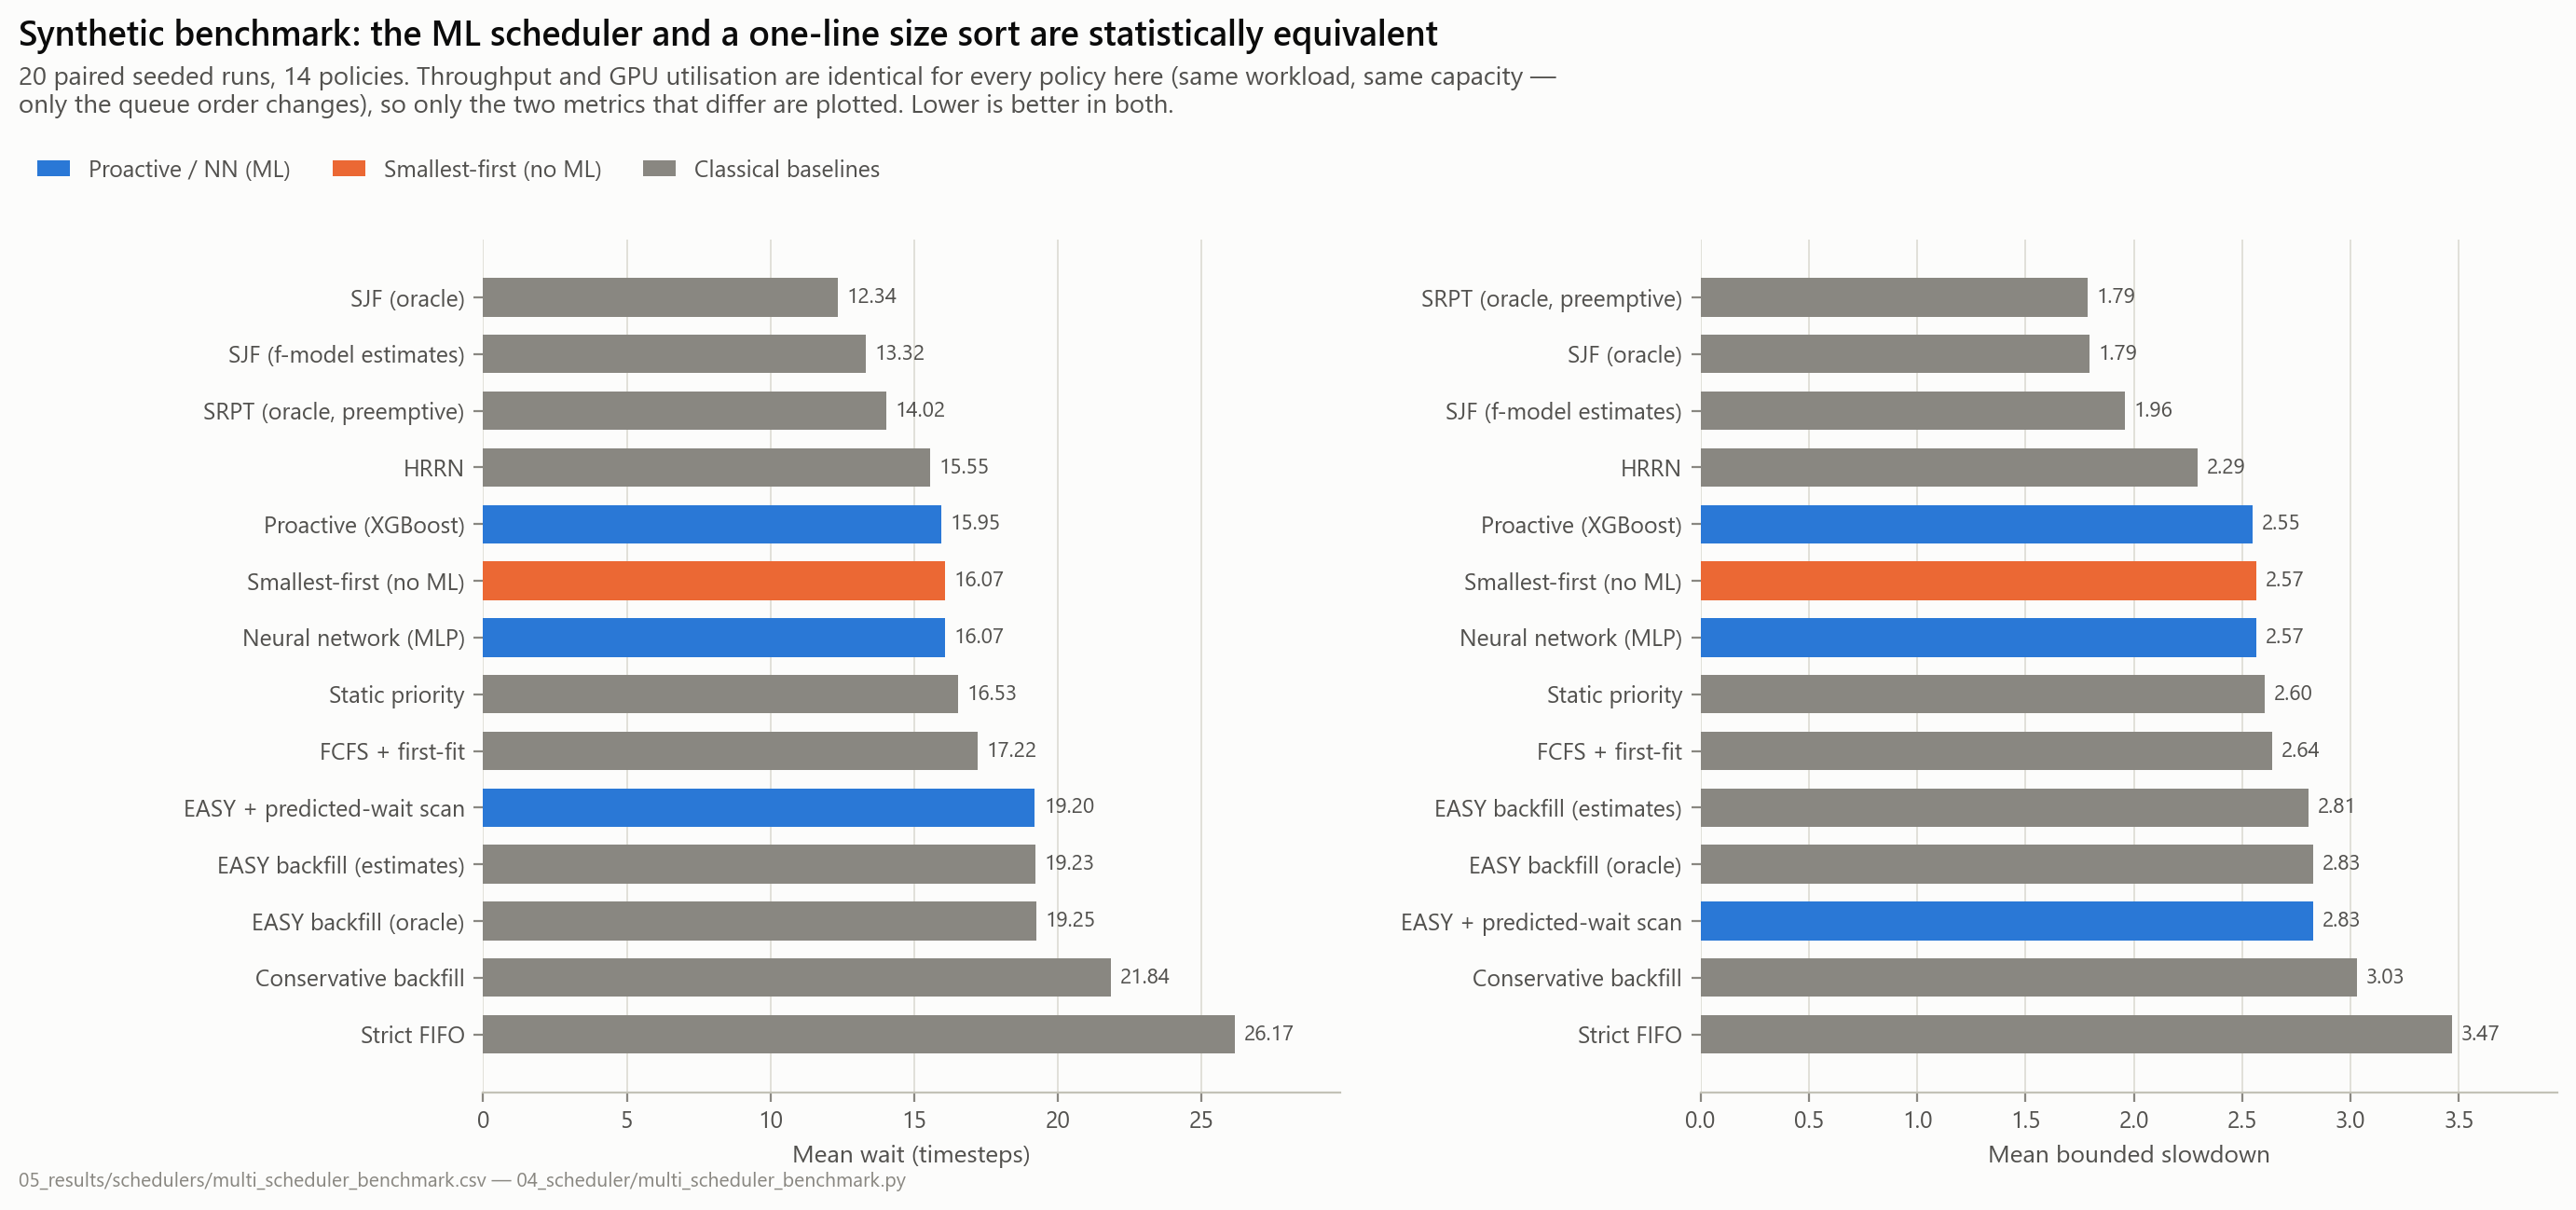
\includegraphics[width=\columnwidth]{../../05_results/schedulers/scheduler_comparison.png}
\caption{Fourteen schedulers on the synthetic substrate, 20 paired runs.
What to look for: the \textsc{Nn} and \textsc{Smallest} bars are not merely
close but the same height --- both sit at $16.074545$ ts mean wait, bit-identical
on every metric of all 20 runs --- and \textsc{Proactive} at $15.9477$ ts is a
hair's breadth from them, inside the $\pm1.59$ ts equivalence margin. The
ML-free sort is not a weak baseline the model narrowly beats; it is where two
different model classes land.
{\small Source:
\texttt{05\_results/schedulers/scheduler\_comparison.png}, plotted from
\texttt{05\_results/schedulers/multi\_scheduler\_benchmark.csv} and
\texttt{05\_results/schedulers/multi\_scheduler\_runs.csv}, produced by
\texttt{python 04\_scheduler/multi\_scheduler\_benchmark.py} (step 7 of
\texttt{run\_all\_experiments.sh}).}}
\label{fig:synth-schedulers}
\end{figure}

On LANL the equivalence test does not fire, and the honest verdict there is
\emph{inconclusive} rather than ``different''. The size sort is $14.4\%$ worse on
mean wait, but that difference does not survive Holm correction on the paired
$t$-test ($p = 0.25$; the Wilcoxon test disagrees at $p = 0.015$), it shrinks to
$+7.3\%$ and $p = 0.60$ on bounded slowdown, and TOST cannot certify equivalence
either ($p = 0.77$). With 20 windows we can neither declare the two policies the
same on LANL nor establish that they differ.

We initially attributed this to the learned size table being less monotone on
LANL, and that explanation is wrong: the per-instant monotone fraction is
$57.1\%$ on SDSC --- where equivalence \emph{does} hold --- against $56.9\%$ on
LANL. Monotonicity does not track where the equivalence fires, so we report the
LANL result as underpowered rather than mechanistically explained. What is not in
question on either machine is the degeneracy itself (\S\ref{sec:degeneracy}), and
on LANL the ML scheduler also fails to beat plain FCFS ($p = 0.48$,
\S\ref{sec:traces}).

\section{Trace-Driven Re-Evaluation}
\label{sec:traces}

Table~\ref{tab:traces} reports the twelve policies on both traces, and
Figure~\ref{fig:trace-comparison} plots them.

\begin{table}[h]
\centering
\small
\begin{tabular}{lrrrr}
\toprule
& \multicolumn{2}{c}{SDSC SP2} & \multicolumn{2}{c}{LANL CM-5} \\
\cmidrule(lr){2-3}\cmidrule(lr){4-5}
Policy & wait & bsld & wait & bsld \\
\midrule
\textsc{Srpt\_Oracle}    &  60.1 &   1.1 &  14.6 &  1.1 \\
\textsc{Sjf\_Oracle}     & 110.8 &  13.2 &  23.0 &  2.8 \\
\textsc{Sjf\_UserEst}    & 115.8 &  14.7 &  31.5 &  4.5 \\
\textsc{Hrrn\_UserEst}   & 126.3 &  16.8 &  29.5 &  5.0 \\
\textsc{Proactive\_Est}  & 125.0 &  14.7 &  37.0 &  5.8 \\
\textsc{Smallest\_First} & 145.0 &  19.0 &  42.5 &  6.6 \\
\textsc{Proactive}       & 145.0 &  18.5 &  37.2 &  6.1 \\
\textsc{FCFS}            & 174.6 &  34.7 &  38.8 &  8.2 \\
\textsc{Easy\_Oracle}    & 183.7 &  35.7 &  46.0 &  8.5 \\
\textsc{Easy\_UserEst}   & 195.1 &  42.5 &  80.2 & 20.6 \\
\textsc{Cons\_Bf\_UserEst}& 207.5 &  40.5 & 113.6 & 28.4 \\
\textsc{Fifo\_Strict}    & 755.1 & 281.5 & 205.7 & 71.4 \\
\bottomrule
\end{tabular}
\caption{Mean wait (minutes) and mean bounded slowdown, averaged over 20 paired
7-day windows per trace at offered load $\approx 0.70$.
{\small Source: \texttt{05\_results/trace\_schedulers/trace\_scheduler\_summary.csv},
produced by \texttt{python 04\_scheduler/trace\_driven\_benchmark.py} (step 10
of \texttt{run\_all\_experiments.sh}).}}
\label{tab:traces}
\end{table}

\begin{figure*}[t]
\centering
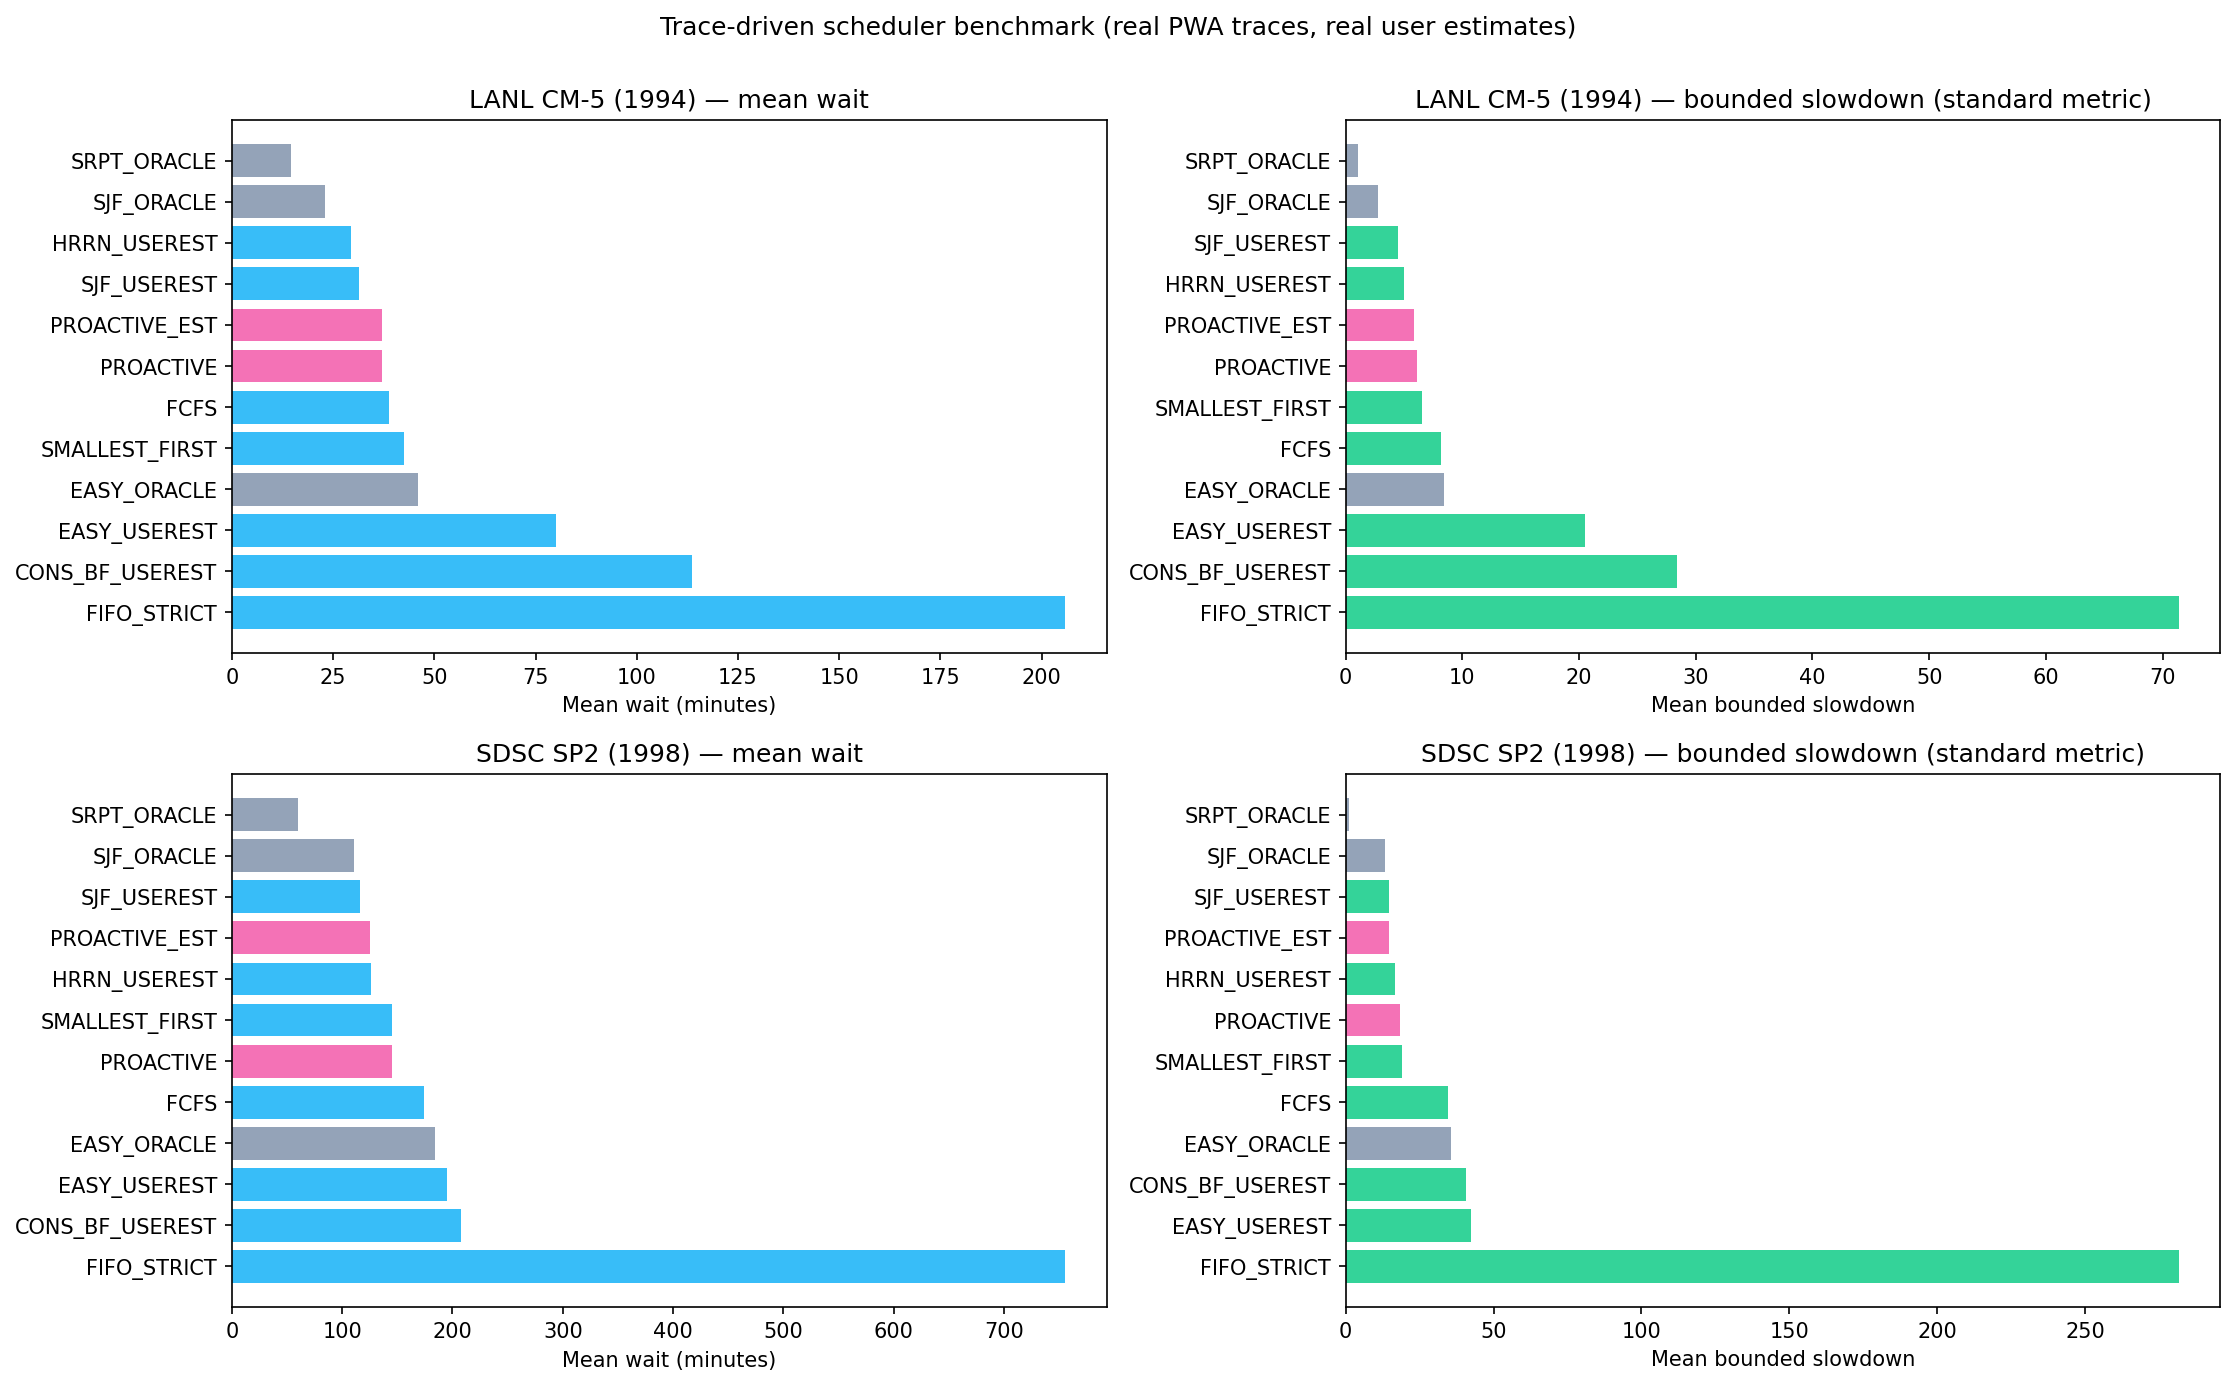
\includegraphics[width=\textwidth]{../../05_results/trace_schedulers/trace_scheduler_comparison.png}
\caption{Twelve policies replayed through two real traces.
What to look for: the \textsc{Proactive} (ML) and \textsc{Smallest\_First}
(ML-free) bars sit next to each other at the same height on SDSC ($145.0$ versus
$145.0$ min mean wait), which is the equivalence of \S\ref{sec:equivalence} seen
directly; and every classical policy holding a runtime estimate --- the
\textsc{Sjf}, \textsc{Hrrn} and oracle bars --- finishes to the left of the ML
bar on both machines. Note also how much further apart the bounded-slowdown
panel spreads the same policies than the mean-wait panel does.
{\small Source:
\texttt{05\_results/trace\_schedulers/trace\_scheduler\_comparison.png},
plotted from
\texttt{05\_results/trace\_schedulers/trace\_scheduler\_summary.csv},
produced by \texttt{python 04\_scheduler/trace\_driven\_benchmark.py} (step 10
of \texttt{run\_all\_experiments.sh}).}}
\label{fig:trace-comparison}
\end{figure*}

\paragraph{The synthetic gain does not replicate.}
On the synthetic benchmark \textsc{Proactive} beats FCFS by $7.4\%$ (and by
$7.9\%$ in the older 40-run paired study). On SDSC it beats FCFS by $20.4\%$
($p = 0.042$, Holm $0.084$); on LANL the difference is $4.5\%$ in
\textsc{Proactive}'s favour but not distinguishable from zero
($p = 0.48$). A method whose advantage over doing nothing is machine-dependent
and insignificant on one of two real machines is not established.

\paragraph{Any runtime signal dominates.}
\textsc{Sjf\_UserEst} --- shortest-job-first on the estimate the user actually
typed --- beats \textsc{Proactive} by $20.2\%$ on SDSC (Holm $p = 0.009$) and
$15.3\%$ on LANL. This is the same conclusion the synthetic study reached, now
on real workloads with real estimate error.

\paragraph{ML adds nothing on top of the estimate.}
\textsc{Proactive\_Est}, which is given the user estimate as a feature and can
therefore in principle learn everything SJF exploits \emph{plus} the cluster
state, does not beat \textsc{Sjf\_UserEst} on either machine ($+7.9\%$ worse on
SDSC, $+17.5\%$ on LANL). The ML pipeline's ceiling here is the sort it is
trying to learn.

\paragraph{Tails and fairness.}
Bounded slowdown separates the policies far more sharply than mean wait, and in
the same direction: \textsc{Proactive} sits at $18.5$ (SDSC) where
\textsc{Sjf\_UserEst} reaches $14.7$ and \textsc{Srpt\_Oracle} $1.1$. The
reordering policies all buy mean wait with equity (Gini $0.88$--$0.89$ versus
$0.83$ for FCFS and $0.45$ for strict FIFO), reproducing the trade-off the
earlier versions of this work reported.

\section{Real Estimate Error Versus the $f$-Model}
\label{sec:estimates}

Because SWF records the user's requested time, the traces let us measure
estimate error instead of simulating it. Table~\ref{tab:est} contrasts the two
machines with the $f$-model at $C = 5$ that our synthetic study (and much of the
backfill literature) assumes.

\begin{table}[h]
\centering
\small
\begin{tabular}{lrrr}
\toprule
 & SDSC & LANL & $f$-model \\
\midrule
Estimate present      & 99.9\% & 90.8\% & --- \\
Median $\hat r / r$   & 6.91 & 1.51 & 3.00 \\
Mean $\hat r / r$     & 61.4 & 23.8 & 3.00 \\
Within $2\times$      & 24.0\% & 41.7\% & --- \\
\textbf{Under-estimates} & 0.1\% & \textbf{36.3\%} & \textbf{0\%} \\
\bottomrule
\end{tabular}
\caption{Real user runtime estimates versus the standard $f$-model.
{\small Source:
\texttt{05\_results/trace\_schedulers/trace\_estimate\_quality.csv},
produced by \texttt{python 04\_scheduler/trace\_driven\_benchmark.py} (step 10
of \texttt{run\_all\_experiments.sh}).}}
\label{tab:est}
\end{table}

The two machines occupy opposite regimes and neither is the $f$-model. SDSC is
extreme over-estimation (median $6.9\times$, nearly no under-estimates); LANL is
roughly calibrated at the median but with a third of jobs under-estimated. The
$f$-model, being $\hat r = r \cdot U(1, C)$, cannot produce an under-estimate at
all.

This is not a cosmetic difference. Our synthetic study concluded that EASY is
``nearly insensitive to estimate quality'' (mean wait $19.0$--$19.8$ ts across
perfect, $f$-model, and modal estimates). On the traces, EASY with real
estimates costs $+6.2\%$ mean wait versus perfect estimates on SDSC --- but
$+74\%$ on LANL (paired $t$ $p = 0.025$ raw but $0.23$ after Holm; the Wilcoxon
signed-rank test over the same 20 windows gives Holm $p = 2.1 \times 10^{-5}$, so the
effect survives correction under the rank test and not under the $t$-test --- the
wait distribution's tail is what carries it). Under-estimates break the mechanism EASY depends
on: a job that claims it will finish before the reservation and does not
\emph{does} delay the head, so the guarantee the reservation is supposed to
provide fails exactly when it matters. An evaluation using only over-estimate
noise cannot observe this. We therefore think the $f$-model should not be used
as the sole estimate-error model in backfill studies.

\section{What Would Make Learning Matter}
\label{sec:fix}

The degeneracy is a property of the feature set, not of XGBoost. A wait-time
model can only produce a non-degenerate ranking if its features distinguish
co-queued jobs by something other than requested size. Concretely, the feature
vector must contain at least one per-job attribute that is (a) not a function of
size given the state, and (b) predictive of wait. Candidates: a runtime estimate
(which is precisely what SJF uses, and which \S\ref{sec:traces} shows the model
then merely reproduces); job-level history such as the submitting user's recent
runtimes; queue/partition identity; dependency structure; or interaction terms
between a per-job attribute and the state (e.g.\ predicted fit against the
future capacity profile rather than the current one).

More broadly, we suggest two evaluation practices. First, \textbf{report the
ML-free control that the model's own feature set implies}: if only the size
feature varies across the queue, the control is sorting by size, and FIFO is not
an adequate comparison. Second, \textbf{use equivalence tests} when arguing that
a component matters --- had we only run difference tests, the Holm-adjusted
$p = 0.17$ comparison between the size sort and the XGBoost pipeline would have
been reported as ``no significant difference'' and quietly dropped, rather than
as the finding it is.

\section{Threats to Validity}
\label{sec:threats}

\paragraph{Reproducibility, and what is platform-dependent.}
Every artefact behind this paper is regenerated by a single committed pipeline,
and two verifiers check it: one re-runs the pipeline in a scratch copy and diffs
every artefact digit for digit, the other asserts the claims themselves. The
distinction is not cosmetic. XGBoost's histogram construction reduces floating
point in parallel, so the fitted model depends on the thread count and library
build of the machine that trained it; the model orders dispatch decisions, so a
different machine visits slightly different instants. A second platform (a
2-vCPU Linux runner) therefore records $45{,}268$ dispatch instants where the
reference platform records $45{,}432$ --- and \emph{zero} counterexamples on
both. Instant counts in this paper should be read as reference-platform figures.
The degeneracy itself is not a platform-dependent quantity, and Proposition~1
says why: it constrains the feature map, not the arithmetic, so any score
computed from per-job inputs that are functions of size given the state is such
a function in any float order. We regard the disagreement in the counts, with
agreement in the result, as corroboration rather than as a defect.

\paragraph{Simulator fidelity, and the measured gap.}
Our trace simulator models \emph{capacity only}. It omits node-level placement
and site policy (partitions, per-user limits, administrative holds), none of
which SWF records, and above all it does not model the real scheduler's policy:
it replays the real arrivals, sizes, runtimes and estimates through our own
FCFS, not through the queue the site actually ran. Averaged over the 20 windows
of each trace, simulated FCFS mean wait is $38.82$ min on LANL against $33.25$
min recorded --- close, and slightly \emph{pessimistic} --- but $174.62$ min on
SDSC against $630.92$ min recorded. We state the SDSC gap plainly: on that trace
the simulator is optimistic by more than a factor of three. (The recorded SDSC
\emph{median} is $19.32$ min, so the recorded mean is carried by an extreme tail
that a capacity-only model has no mechanism to reproduce; that explains the gap
but does not close it.) SDSC results should therefore be read as ``a
correctly-loaded 128-processor machine driven by the real arrival, size, runtime
and estimate distributions'', not as a replay of SDSC's actual queue, and any
absolute SDSC wait figure in this paper should be discounted accordingly. What
survives the gap is the \emph{relative} comparison, since all twelve policies
run in the same simulator on the same windows, and the degeneracy result, which
is a property of the feature vector rather than of the simulator and holds in
all three substrates.

\paragraph{Synthetic workload realism.}
One of our three settings is a synthetic generator, and it is not a validated
workload model: 8 nodes $\times$ 4 GPUs, uniform arrivals, sizes $U\{1,8\}$,
runtimes $U\{5,20\}$, chosen for continuity with earlier versions of this work
rather than for fidelity to any machine. Lublin and Feitelson
\cite{Lublin2003}, Downey and Feitelson \cite{Downey1999}, and Feitelson and
Shmueli \cite{Feitelson2009} describe what a principled generator would look
like, and ours is none of those. Of the $45{,}432$ dispatch instants behind the
zero-counterexample count, $3{,}646$ come from this generator and $41{,}786$
from the two real traces; the synthetic arm is thus the smaller share, but it is
not negligible. It is also the \emph{weaker} arm in a second respect: the Phase D
adversarial attacks of \S\ref{sec:scope} were run against the two traces only,
so the synthetic setting has been measured but not attacked. Readers should
treat the trace evidence as primary and the synthetic evidence as corroborating.

\paragraph{Statistical power, and one test that cannot be settled.}
Twenty windows per trace gives limited power; after Holm correction across the
family of eleven comparisons many individually plausible differences are not
significant, particularly on LANL. The LANL mean-wait equivalence test between
\textsc{Smallest\_First} and \textsc{Proactive} is the sharpest case, and it is
worse than merely underpowered: its achieved power is $0.47\%$, and because the
observed difference ($320.02$ s) \emph{exceeds} the equivalence margin
($222.93$ s), TOST power falls toward zero as $n$ grows --- \emph{no} sample
size can certify equivalence there at a $10\%$ margin. Establishing a
\emph{difference} instead would need $29$ windows, or $50$ after Holm correction
over the family of eleven, and LANL supplies only $28$ disjoint 7-day windows.
The LANL row is therefore \textbf{inconclusive}, not ``different'', and it
cannot be settled on that trace at all; settling it requires a different or
longer trace. We say this rather than reporting the failed equivalence test as
evidence of a difference, which is the error the paper's own methodology section
warns against. Elsewhere we lean on effect sizes, on the consistency of the
ordering across both machines, and --- for the sameness claims --- on
equivalence tests rather than on failures to reject.
{\small Source:
\texttt{05\_results/trace\_schedulers/tost\_power.csv}, produced by
\texttt{python 04\_scheduler/tost\_power.py} (step 11 of
\texttt{run\_all\_experiments.sh}).}

\paragraph{Which model split the accuracy number comes from.}
The wait model's headline accuracy in this paper is the run-wise grouped split:
$R^2 = 0.810910 \pm 0.020672$ and MAE $4.8970$ over five GroupKFold folds on the
run identifier. Earlier versions of this work quoted a uniformly random
row-level split, $R^2 = 0.836840$ and MAE $4.6935$, which is optimistic: the
$2{,}200$ rows are 20 simulation runs of 110 jobs each, so a random split puts
rows of the same run --- and adjacent instants of it --- on both sides. Under a
within-run \emph{chronological} split, which is what deployment actually means
(train on a run's earlier arrivals, predict its later ones), $R^2$ falls to
$0.725147$ and MAE rises to $7.2403$. We report the run-wise figure as the
headline and the chronological figure as the deployment bound. None of this
touches the degeneracy result: that result is a statement about the
\emph{functional form} of the score --- that it factors through requested size
--- and it holds for a perfect model exactly as it holds for a poor one. This
caveat bounds the deployment story, not the contribution.
{\small Source: \texttt{05\_results/models/evaluation\_splits.csv}, produced by
\texttt{python 03\_models/evaluate\_splits.py} (step 23 of
\texttt{run\_all\_experiments.sh}).}

\paragraph{Covariate shift in the retrained model.}
The per-trace model is trained on features reconstructed from the \emph{recorded}
schedule, produced by the site's real scheduler. When \textsc{Proactive} runs it
induces different states than those it was trained on. This is inherent to the
approach rather than an artefact of our setup, but it means the model is
evaluated slightly off-distribution even after retraining.

\paragraph{Vintage of the traces.}
LANL CM-5 (1994) and SDSC SP2 (1998) are batch HPC machines. Their users supply
runtime estimates, which is exactly the regime in which the ML scheduler has no
niche. Modern deep-learning clusters, where job durations are often genuinely
unknown at submit time, are the setting in which a zero-runtime-information
policy could still be worth something; validating there is the clearest next
step, and we make no claim about it here.

\paragraph{The scope of the negative result.}
\label{sec:scope}
This is a negative result about \emph{one feature family}, not about ML
scheduling in general, and we want the boundary to be unmistakable. The claim is:
\emph{a score computed at the dispatch instant, over features that consist of
cluster state plus per-job attributes that factor through requested size given
that state, cannot rank two co-queued jobs of equal size.} Everything outside
that description is untouched.

We tested the boundary in both directions. In the converse direction, adding
per-job attributes that are genuinely not functions of size given the state ---
the user's runtime estimate, causal per-user history, queue identity, user
identity --- breaks the degeneracy immediately: counterexample counts rise from
$0$ to between $6{,}194$ and $10{,}718$ on SDSC and from $0$ to between
$13{,}801$ and $28{,}497$ on LANL, across five such attributes each of which
breaks it on its own. Breaking the degeneracy is not the same as scheduling
better, however: $0$ of the $12$ augmented variants beat \textsc{Sjf\_UserEst},
and the best of them (LANL with all attributes added) is $1.48\%$ \emph{slower}
than that plain sort and TOST-equivalent to it ($p = 0.0014$).

In the adversarial direction, we attacked the claim itself. A pairwise
learning-to-rank objective (\texttt{rank:pairwise}), a listwise one
(\texttt{rank:ndcg}), monotone score transforms (\texttt{log1p} and a sigmoid),
and a 5-tick lagged history window all yield \emph{zero} counterexamples: the
degeneracy is a property of the feature map, and changing the loss or
monotonically reshaping the score does not touch it. One attack does break the
claim, and it breaks it by violating the premise rather than by evading the
argument: scoring a job when it \emph{enters} the queue and caching that score
gives $20{,}482$ (SDSC) and $37{,}741$ (LANL) counterexamples, because two
equally-sized jobs then carry scores computed against \emph{different} cluster
states. This is the shared-state assumption failing by construction, and it is
why we scope the claim to a score computed at the dispatch instant. It also
costs: enqueue-time caching is worse on LANL ($+11.74\%$ mean wait and $27\%$
worse bounded slowdown) and, while nominally $1.64\%$ better on SDSC mean wait,
raises SDSC median wait from $76.0$ to $105.4$ s and bounded slowdown from
$18.49$ to $21.56$.
{\small Source:
\texttt{05\_results/degeneracy/non\_degeneracy\_sweep.csv} and
\texttt{05\_results/degeneracy/non\_degeneracy\_utility.csv}, produced by
\texttt{python 04\_scheduler/non\_degeneracy\_sweep.py} (step 12 of
\texttt{run\_all\_experiments.sh}); and
\texttt{05\_results/degeneracy/robustness\_attacks.csv} and
\texttt{05\_results/degeneracy/robustness\_attack\_utility.csv}, produced by
\texttt{python 04\_scheduler/robustness\_attacks.py} (step 13).}

\section{Conclusion}

We set out to find where an ML wait-time scheduler adds value and found that,
as constructed, it cannot add value to queue ordering: its score is a function
of requested size alone, verified over $45{,}432$ dispatch instants without a
single counterexample. A one-line sort is statistically equivalent to it on two
of three substrates, an MLP over the same features reproduces the sort exactly,
its synthetic advantage over FCFS does not replicate on real traces, and any
classical policy holding a runtime estimate beats it on both real machines.
Alongside this we report that real user-estimate error damages backfill far more
than the standard $f$-model predicts, because a third of LANL's estimates are
under-estimates that the $f$-model cannot generate.

We report these as negative results because they are the results. The
constructive content is the non-degeneracy condition of \S\ref{sec:fix} and the
methodological point that an ML systems component should be compared against the
ML-free control its own feature set implies --- with an equivalence test, not a
failed difference test.

\section*{Artifact Availability}
Code, both SWF traces, the seeded pipeline
(\texttt{run\_all\_experiments.sh}), and every CSV behind the tables are in the
repository. \texttt{04\_scheduler/ranking\_degeneracy.py} reproduces
\S\ref{sec:degeneracy}, \texttt{trace\_driven\_benchmark.py} reproduces
\S\ref{sec:traces}--\ref{sec:estimates}, and
\texttt{multi\_scheduler\_benchmark.py} reproduces \S\ref{sec:equivalence}.

\begin{thebibliography}{99}

\bibitem{Feitelson1997} D. G. Feitelson, \emph{Workload Modeling for Job Scheduling in Parallel Computers}, EWOPP 1997.

\bibitem{SLURM2003} A. Yoo et al., \emph{SLURM: Simple Linux Utility for Resource Management}, JSSPP 2003.

\bibitem{Jain1984} R. Jain, D.-M. Chiu, and W. Hawe, \emph{A Quantitative Measure of Fairness and Discrimination for Resource Allocation in Shared Computer Systems}, DEC Research Report TR-301, 1984.

\bibitem{Feitelson2000} D. G. Feitelson, \emph{Metrics for Parallel Job Scheduling and Their Convergence}, JSSPP 2001.

\bibitem{Feitelson2011} D. G. Feitelson, D. Tsafrir, and D. Krakov, \emph{Experience with Using the Parallel Workloads Archive}, J. Parallel Distrib. Comput. 74(10):2967--2982, 2014. \url{https://www.cs.huji.ac.il/labs/parallel/workload/}

\bibitem{Mualem2001} A. W. Mu'alem and D. G. Feitelson, \emph{Utilization, Predictability, Workloads, and User Runtime Estimates in Scheduling the IBM SP2 with Backfilling}, IEEE TPDS 12(6), 2001.

\bibitem{Tsafrir2005} D. Tsafrir, Y. Etsion, and D. G. Feitelson, \emph{Modeling User Runtime Estimates}, JSSPP 2005.

\bibitem{ML-Scheduling1} H. Mao, M. Alizadeh, I. Menache, and S. Kandula, \emph{Resource Management with Deep Reinforcement Learning}, HotNets 2016.

\bibitem{ML-Scheduling2} H. Mao, M. Schwarzkopf, S. B. Venkatakrishnan, Z. Meng, and M. Alizadeh, \emph{Learning Scheduling Algorithms for Data Processing Clusters}, SIGCOMM 2019.


\bibitem{Tsafrir2007} D. Tsafrir, Y. Etsion, and D. G. Feitelson, \emph{Backfilling Using System-Generated Predictions Rather Than User Runtime Estimates}, IEEE TPDS 18(6):789--803, 2007.

\bibitem{Nissimov2007} A. Nissimov and D. G. Feitelson, \emph{Probabilistic Backfilling}, JSSPP 2007.

\bibitem{Shmueli2003} E. Shmueli and D. G. Feitelson, \emph{Backfilling with Lookahead to Optimize the Packing of Parallel Jobs}, JSSPP 2003.

\bibitem{Shmueli2005} E. Shmueli and D. G. Feitelson, \emph{Backfilling with System-Generated Job Runtime Estimates}, IPDPS 2005.

\bibitem{Talby1999} D. Talby and D. G. Feitelson, \emph{Supporting Priorities and Improving Utilization of the IBM SP Scheduler Using Slack-Based Backfilling}, IPPS/SPDP 1999.

\bibitem{Feitelson2005} D. G. Feitelson, \emph{Experimental Analysis of the Root Causes of Performance Evaluation Results: A Backfilling Case Study}, IEEE TPDS 16(2):175--182, 2005.

\bibitem{Hai2023} T. H. L. Hai, K. N. Duy, T. N. Manh, D. M. Hoang, and N. Thoai, \emph{Deviation Backfilling: A Robust Backfilling Scheme for Improving the Efficiency of Job Scheduling on High Performance Computing Systems}, IEEE, 2023.

\bibitem{Minh2010} T. N. Minh and L. Wolters, \emph{Using Historical Data to Predict Application Runtimes on Backfilling Parallel Systems}, IEEE, 2010.

\bibitem{Yuan2014} Y. Yuan, Y. Wu, W. Zheng, and K. Li, \emph{Guarantee Strict Fairness and Utilize Prediction Better in Parallel Job Scheduling}, IEEE TPDS, 2014.

\bibitem{Park2019} J.-W. Park, \emph{Queue Waiting Time Prediction for Large-scale High-performance Computing System}, IEEE, 2019.

\bibitem{Park2025} J.-W. Park and T. Hong, \emph{Improving Runtime Prediction Performance Based on Application Type of Jobs on Large-scale Cluster System}, IEEE, 2025.

\bibitem{Lovell2024} A. Lovell, P. Wisniewski, S. Rodenbeck, et al., \emph{A Hierarchical Deep Learning Approach for Predicting Job Queue Times in HPC Systems}, IEEE, 2024.

\bibitem{Ramachandran2024} S. Ramachandran, M. L. Jayalal, et al., \emph{Combining Machine Learning and Metaheuristic Algorithms for Predicting Waiting Time of High Performance Computing Jobs}, IEEE, 2024.

\bibitem{Barsanti2006} L. Barsanti and A. C. Sodan, \emph{Adaptive Job Scheduling via Predictive Job Resource Allocation}, JSSPP 2006.

\bibitem{Wang2023} H. Wang, Z. Liu, and H. Shen, \emph{Machine Learning Feature Based Job Scheduling for Distributed Machine Learning Clusters}, IEEE/ACM Trans. Networking 31(1):58--72, 2023.

\bibitem{Hovestadt2003} M. Hovestadt, O. Kao, A. Keller, and A. Streit, \emph{Scheduling in HPC Resource Management Systems: Queuing vs. Planning}, JSSPP 2003.

\bibitem{Lublin2003} U. Lublin and D. G. Feitelson, \emph{The Workload on Parallel Supercomputers: Modeling the Characteristics of Rigid Jobs}, J. Parallel Distrib. Comput. 63(11):1105--1122, 2003.

\bibitem{Downey1999} A. B. Downey and D. G. Feitelson, \emph{The Elusive Goal of Workload Characterization}, ACM SIGMETRICS Perf. Eval. Rev. 26(4):14--29, 1999.

\bibitem{Feitelson2009} D. G. Feitelson and E. Shmueli, \emph{A Case for Conservative Workload Modeling: Parallel Job Scheduling with Daily Cycles of Activity}, MASCOTS 2009.

\bibitem{Zhang2024} D. Zhang, M. S. Raj, B. Xie, S. Di, and D. Dai, \emph{Cross-System Analysis of Job Characterization and Scheduling in Large-Scale Computing Clusters}, IEEE, 2024.

\bibitem{Burges2005} C. Burges, T. Shaked, E. Renshaw, A. Lazier, M. Deeds, N. Hamilton, and G. Hullender, \emph{Learning to Rank Using Gradient Descent}, ICML 2005.

\bibitem{Liu2009} T.-Y. Liu, \emph{Learning to Rank for Information Retrieval}, Foundations and Trends in Information Retrieval 3(3):225--331, 2009.

\bibitem{Kraska2018} T. Kraska, A. Beutel, E. H. Chi, J. Dean, and N. Polyzotis, \emph{The Case for Learned Index Structures}, SIGMOD 2018.

\bibitem{Marcus2020} R. Marcus, A. Kipf, A. van Renen, M. Stoian, S. Misra, A. Kemper, T. Neumann, and T. Kraska, \emph{Benchmarking Learned Indexes}, Proc. VLDB Endowment 14(1):1--13, 2020.

\bibitem{Armstrong2009} T. G. Armstrong, A. Moffat, W. Webber, and J. Zobel, \emph{Improvements That Don't Add Up: Ad-Hoc Retrieval Results Since 1998}, CIKM 2009.

\bibitem{Lin2018} J. Lin, \emph{The Neural Hype and Comparisons Against Weak Baselines}, ACM SIGIR Forum 52(2):40--51, 2018.

\bibitem{Dacrema2019} M. Ferrari Dacrema, P. Cremonesi, and D. Jannach, \emph{Are We Really Making Much Progress? A Worrying Analysis of Recent Neural Recommendation Approaches}, RecSys 2019.

\bibitem{Musgrave2020} K. Musgrave, S. Belongie, and S.-N. Lim, \emph{A Metric Learning Reality Check}, ECCV 2020.

\bibitem{Sculley2018} D. Sculley, J. Snoek, A. Wiltschko, and A. Rahimi, \emph{Winner's Curse? On Pace, Progress, and Empirical Rigor}, ICLR 2018 Workshop Track.

\bibitem{Collberg2016} C. Collberg and T. A. Proebsting, \emph{Repeatability in Computer Systems Research}, Communications of the ACM 59(3):62--69, 2016.

\bibitem{Goponenko2022} A. V. Goponenko, K. Lamar, C. Peterson, B. A. Allan, J. M. Brandt, and D. Dechev, \emph{Metrics for Packing Efficiency and Fairness of HPC Cluster Batch Job Scheduling}, IEEE, 2022.

\end{thebibliography}

\end{document}
